\documentclass[12pt, a4paper]{article}
% --- Codificación y lenguaje ---
\usepackage[utf8]{inputenc}
\usepackage[T1]{fontenc}
\usepackage[spanish]{babel}

% --- Márgenes ---
\usepackage[top=2.5cm, bottom=2.5cm, left=3cm, right=2.5cm]{geometry}

% --- Tipografía ---
\usepackage{lmodern}

% --- Matemáticas ---
\usepackage{amsmath}
\usepackage{amssymb}

% --- Figuras y tablas ---
\usepackage{graphicx}
\usepackage{booktabs}
\usepackage{float}
\usepackage{caption}
\usepackage{subcaption}

% --- Colores ---
\usepackage{xcolor}

% --- Hipervínculos ---
\usepackage[colorlinks=true, linkcolor=blue, citecolor=blue, urlcolor=blue]{hyperref}

% --- Interlineado ---
\usepackage{setspace}
\onehalfspacing

% --- Encabezados y pies de página ---
\usepackage{fancyhdr}
\pagestyle{fancy}
\fancyhf{}
\lhead{\small Región Andina occidental (1996--2025)}
\rhead{\small Mini Proyecto 2}
\rfoot{\thepage}

% --- Bibliografía ---
\usepackage[numbers, sort&compress]{natbib}

% =============================================================
\begin{document}
	
	\begin{titlepage}
		\centering
		\vspace*{2cm}
		{\LARGE \textbf{Mini Proyecto 2: Dinámica y termodinámica atmosférica regional}\\[0.5em]
			\large Atmósfera estándar, climatologías de reanálisis\\
			y aproximación geostrófica (1996--2025)}\\[2cm]
		{\large Jhon García Barrera}\\[0.5em]
		{\normalsize Física del Clima y Cambio Climático}\\[0.5em]
		{\normalsize \today}\\[3cm]
		\vfill
		{\small Código y datos disponibles en:\\
			\url{https://github.com/jhongarciab/proyectos-clima/tree/main/proyecto%202}}
	\end{titlepage}
	
	\tableofcontents
	\newpage

\section{Introducción}
\label{sec:intro}
% ============================================================

La atmósfera terrestre es un fluido estratificado cuyo comportamiento
dinámico y termodinámico puede describirse, en primera aproximación,
mediante un conjunto de ecuaciones idealizadas que capturan las
relaciones fundamentales entre presión, temperatura y densidad.
Entre estas aproximaciones, la Atmósfera Estándar Internacional
(ISA, \textit{International Standard Atmosphere}) constituye el modelo
de referencia más ampliamente adoptado, tanto en aviación como en
estudios climáticos y comparaciones instrumentales
\citep{iso1975standard}.

El presente trabajo tiene como objetivo evaluar la validez y las
limitaciones de tres de estas aproximaciones en el contexto de una
región de estudio concreta: el Eje Cafetero colombiano.
Esta región se caracteriza por una topografía compleja dominada por
las cordilleras Central y Occidental de los Andes, elevaciones que
oscilan entre los $700$ y los $3\,000$\,m sobre el nivel del mar, y
un régimen climático de tipo bimodal determinado por la migración de
la Zona de Convergencia Intertropical (ZCIT).

Las aproximaciones evaluadas son:

\begin{enumerate}
	\item La \textbf{Atmósfera Estándar ISA}, que describe los perfiles
	verticales de temperatura, presión y densidad mediante leyes
	analíticas basadas en gradientes térmicos constantes por capas
	y la ecuación hidrostática.
	
	\item La \textbf{aproximación geostrófica}, que relaciona el campo
	de viento horizontal con el gradiente horizontal del geopotencial
	bajo el supuesto de equilibrio entre la fuerza de gradiente de
	presión y la fuerza de Coriolis.
	
	\item La \textbf{representación del perfil vertical de temperatura}
	de la región mediante los campos climatológicos del reanálisis ERA5
	y su comparación con el perfil ISA de referencia.
\end{enumerate}

Para llevar a cabo el análisis se emplearon datos del reanálisis ERA5
del Centro Europeo de Predicción Meteorológica a Plazo Medio
(ECMWF, \citealt{hersbach2020era5}), correspondientes al período
1996--2025 en promedios mensuales, tanto en niveles de superficie como
en catorce niveles de presión entre $1\,000$ y $50$\,hPa.
La región de estudio se ilustra en la Figura~\ref{fig:mapa_region},
donde se aprecia su localización en el contexto Colombiano.

\begin{figure}[H]
	\centering
	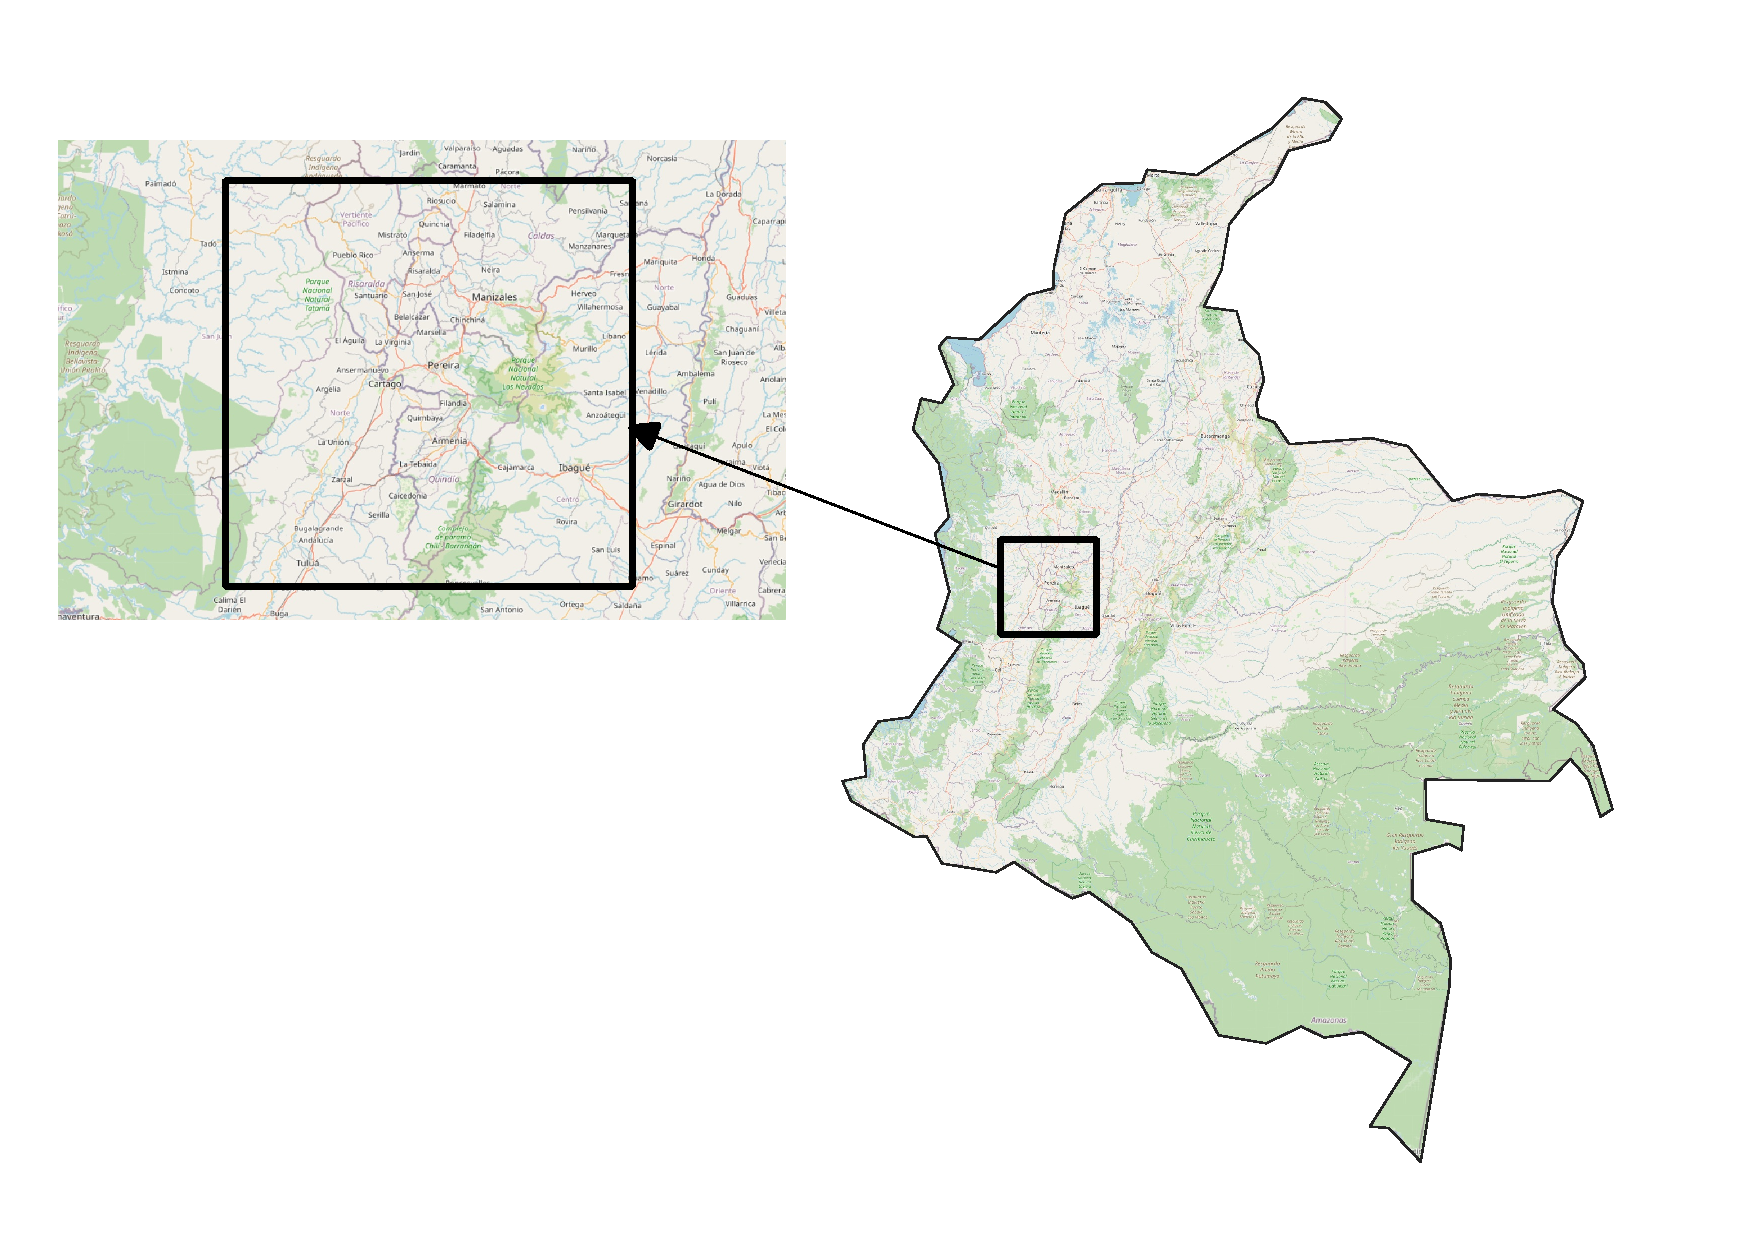
\includegraphics[width=0.70\textwidth]{../../results/plots/mapa.pdf}
	\caption{Localización de la región de estudio sobre
		el mapa de Colombia. La región cubre el Eje Cafetero y parte del
		departamento del Tolima, con coordenadas
		$4.0$--$5.5^{\circ}$\,N y $76.5$--$75.0^{\circ}$\,W.}
	\label{fig:mapa_region}
\end{figure}


% ============================================================
\section{Atmósfera Estándar ISA}
\label{sec:isa}
% ============================================================

\subsection{Fundamento físico}

La Atmósfera Estándar Internacional (ISA, ISO~2533:1975) define un perfil
vertical de referencia para temperatura, presión y densidad del aire seco en
reposo, válido en condiciones promedio de latitudes medias
\citep{iso1975standard}. Su construcción parte de dos relaciones
físicas fundamentales: el equilibrio hidrostático

\begin{equation}
	\frac{dp}{dz} = -\rho\, g_0,
	\label{eq:hidro}
\end{equation}

y la ecuación de estado del gas ideal para aire seco

\begin{equation}
	p = \rho\, R_d\, T,
	\label{eq:ideal}
\end{equation}

donde $g_0 = 9.80665\,\mathrm{m\,s^{-2}}$ es la gravedad estándar,
$R_d = 287.05\,\mathrm{J\,kg^{-1}\,K^{-1}}$ la constante específica del
aire seco, $T$ la temperatura absoluta, $p$ la presión y $\rho$ la
densidad. Sustituyendo~\eqref{eq:ideal} en~\eqref{eq:hidro} se obtiene
la forma separable

\begin{equation}
	\frac{dp}{p} = -\frac{g_0}{R_d\,T(z)}\,dz,
	\label{eq:sep}
\end{equation}

cuya integración depende del perfil térmico $T(z)$ en cada capa.

\subsection{Capas atmosféricas y perfiles analíticos}

La ISA divide la atmósfera en capas con gradiente térmico vertical
$L = dT/dz$ constante. La implementación cubre las siete capas
oficiales de la norma hasta $86$\,km (tope de la mesosfera), que se
listan en la Tabla~\ref{tab:capas_isa}. Se extiende el análisis
completo hasta $86$\,km para contextualizar la estructura termal
global, aunque el foco del trabajo corresponde a la troposfera y la
estratosfera baja ($0$--$20$\,km), que son las capas relevantes para
la dinámica sinóptica de la región de estudio.

\begin{table}[H]
	\centering
	\caption{Capas de la Atmósfera Estándar ISA implementadas
		(ISO~2533:1975). $L$ en $\mathrm{K\,km^{-1}}$;
		$T_\text{base}$ y $p_\text{base}$ son las condiciones
		en el límite inferior de cada capa.}
	\label{tab:capas_isa}
	\small
	\begin{tabular}{lcccc}
		\toprule
		Capa & $z$ (km) & $L$ ($\mathrm{K\,km^{-1}}$)
		& $T_\text{base}$ (K) & Nombre \\
		\midrule
		Troposfera           &   0--11  & $-6.5$ & 288.15 & Troposfera \\
		Estratosfera baja    &  11--20  &  $0.0$ & 216.65 & Est.\ baja \\
		Estratosfera media   &  20--32  & $+1.0$ & 216.65 & Est.\ media \\
		Estratosfera alta    &  32--47  & $+2.8$ & 228.65 & Est.\ alta \\
		Estratopausa         &  47--51  &  $0.0$ & 270.65 & Estratopausa \\
		Mesosfera baja       &  51--71  & $-2.8$ & 270.65 & Mesos.\ baja \\
		Mesosfera alta       &  71--86  & $-2.0$ & 214.65 & Mesos.\ alta \\
		\bottomrule
	\end{tabular}
\end{table}

\paragraph{Capas con gradiente no nulo.}
En una capa de gradiente $L \neq 0$, el perfil de temperatura es lineal:
\begin{equation}
	T(z) = T_\text{base} + L\,(z - z_\text{base}).
	\label{eq:T_lineal}
\end{equation}
Integrando~\eqref{eq:sep} con este perfil y definiendo el exponente
adimensional
\begin{equation}
	\alpha = \frac{g_0}{R_d\,|L|},
	\label{eq:alpha}
\end{equation}
se obtiene la ley de potencia
\begin{equation}
	p(z) = p_\text{base}
	\left(\frac{T(z)}{T_\text{base}}\right)^{-\alpha}.
	\label{eq:p_tropo}
\end{equation}
Para la troposfera, $|L| = 6.5 \times 10^{-3}\,\mathrm{K\,m^{-1}}$ y
$\alpha = g_0 / (R_d\,|L|) \approx 5.256$, valor que gobierna la
variación de presión con la temperatura en toda esta capa.

\paragraph{Capas isotérmicas ($L = 0$).}
Cuando $T = T_\text{base}$ es constante, la ecuación~\eqref{eq:sep}
se integra directamente a una exponencial:
\begin{equation}
	p(z) = p_\text{base}
	\exp\!\left[-\frac{g_0\,(z - z_\text{base})}{R_d\,T_\text{base}}\right].
	\label{eq:p_iso}
\end{equation}
Esta forma es la \textit{fórmula barométrica} y se aplica a la
estratosfera baja ($11$--$20$\,km) y a la estratopausa ($47$--$51$\,km).

\paragraph{Densidad.}
En ambos tipos de capa, la densidad se obtiene algebraicamente de la
ecuación de estado:
\begin{equation}
	\rho(z) = \frac{p(z)}{R_d\,T(z)}.
	\label{eq:rho}
\end{equation}

Las condiciones de base de cada capa se propagan de forma encadenada
desde las condiciones de superficie $T_0 = 288.15$\,K y
$p_0 = 101\,325$\,Pa, garantizando continuidad exacta en todas las
interfaces.

Los perfiles calculados se muestran en la
Figura~\ref{fig:isa_perfiles} para el dominio completo $0$--$86$\,km
y  para el rango $0$--$20$\,km
de interés para este trabajo. Tres rasgos estructurales destacan en
los perfiles: primero, la temperatura exhibe el perfil en ``S'' característico, con
	enfriamiento monótono en la troposfera, inversión cálida en la
	estratosfera alta (máximo en la estratopausa, $\sim\!270$\,K a
	$47$\,km) y nuevo enfriamiento hasta la mesopausa; segundo, la presión y la densidad decaen de forma cuasiexponencial en
	toda la columna, perdiendo aproximadamente un orden de magnitud
	cada $16$\,km. A $86$\,km, la presión es $\sim\!0.004$\,hPa,
	menos de $4\times10^{-6}$ veces la presión superficial; tercero, el eje de presión en las figuras se presenta en escala
	lineal, lo que permite apreciar directamente la forma exponencial
	del decaimiento, equivalente a una recta en escala logarítmica.
	
\begin{figure}[H]
	\centering
	\begin{subfigure}[t]{0.49\textwidth}
		\centering
		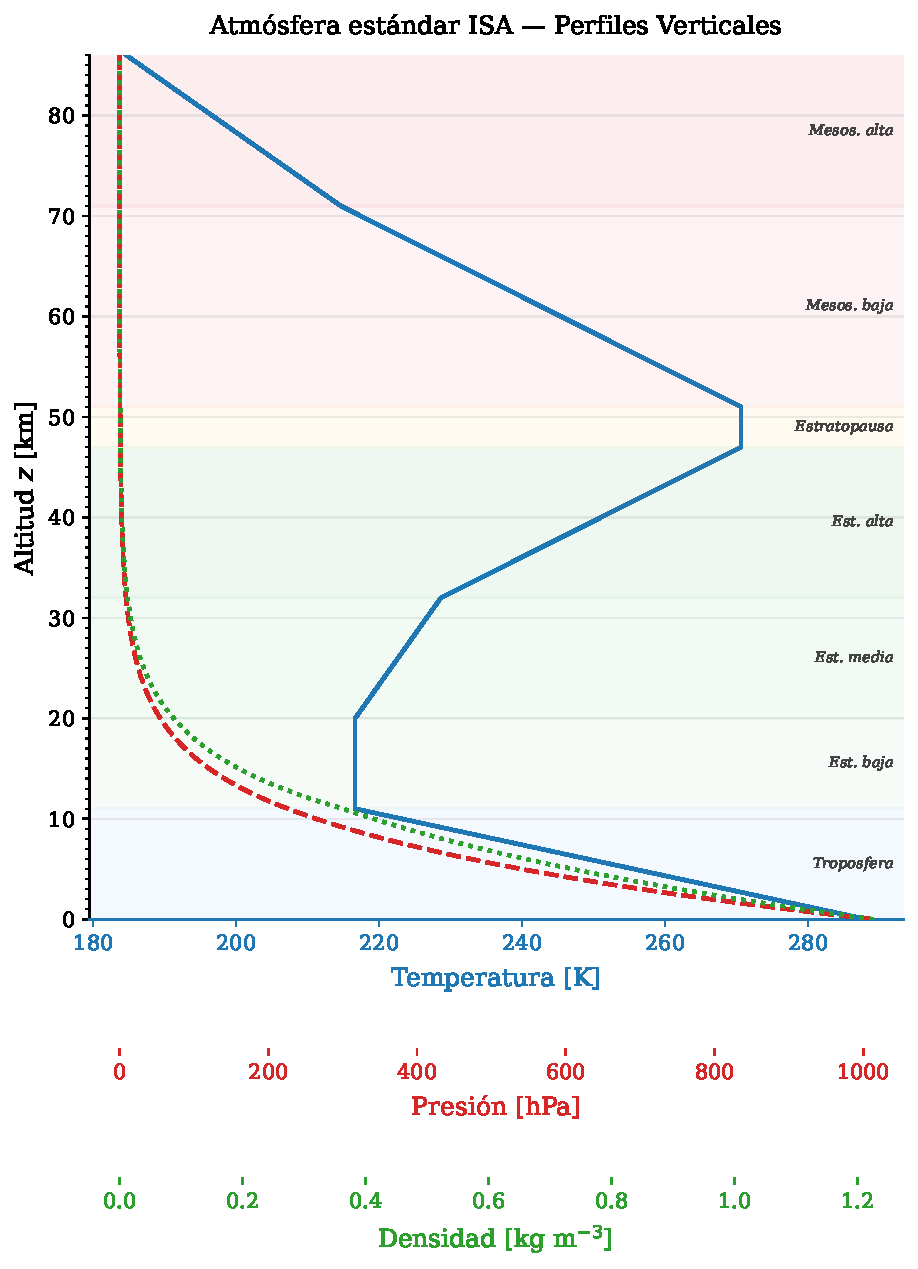
\includegraphics[width=\textwidth]{../../results/plots/01_atmosfera_estandar_full.pdf}
		\caption{Perfil completo entre 0 y 86\,km.}
		\label{fig:isa_perfiles_full}
	\end{subfigure}
	\hfill
	\begin{subfigure}[t]{0.49\textwidth}
		\centering
		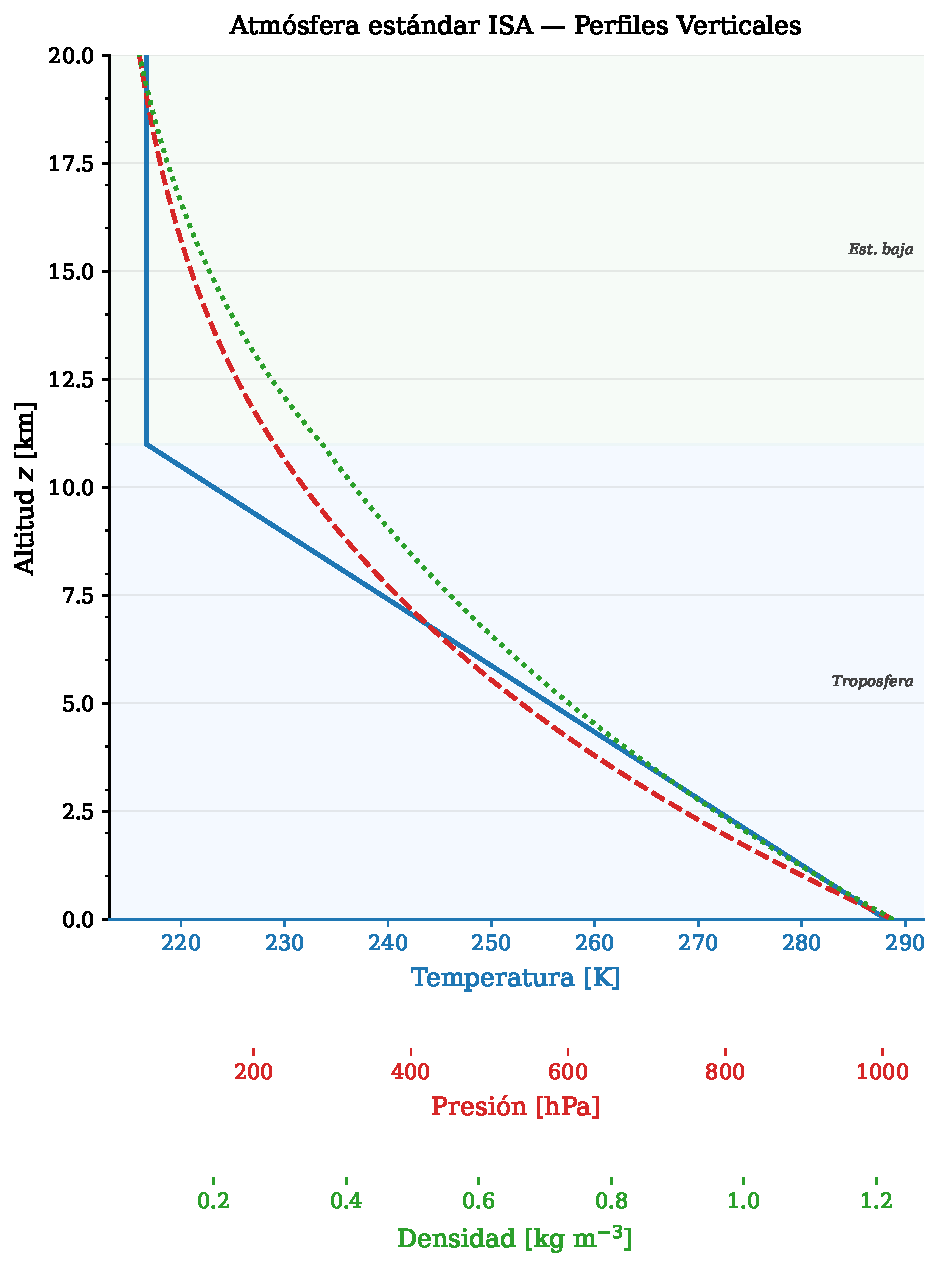
\includegraphics[width=\textwidth]{../../results/plots/01_atmosfera_estandar_zoom.pdf}
		\caption{Detalle entre 0 y 20\,km.}
		\label{fig:isa_perfiles_zoom}
	\end{subfigure}
	\caption{Perfiles verticales de temperatura, presión y densidad para la atmósfera estándar (ISA), mostrando tanto el detalle en la baja atmósfera como la estructura completa de la columna atmosférica.}
	\label{fig:isa_perfiles}
\end{figure}

La implementación se verificó en tres niveles. Primero, se comprobó
la consistencia interna del sistema: el error relativo en el cierre
de la ecuación de estado $|p - \rho R_d T|/p$ es inferior a
$4 \times 10^{-14}$\,\% (esencialmente precisión de máquina), y el
residuo del balance hidrostático calculado por diferencias finitas
tiene un error medio de $5 \times 10^{-3}$\,\%. Segundo, se verificó
la monotonicidad: tanto $p(z)$ como $\rho(z)$ son estrictamente
decrecientes en todo el dominio. Tercero, se compararon los valores
calculados con la tabla oficial ISO~2533:1975 en ocho altitudes clave
(Tabla~\ref{tab:validacion_isa}).

\begin{table}[H]
	\centering
	\caption{Comparación de los perfiles calculados con la tabla
		oficial ISA (ISO~2533:1975). Los errores relativos
		en temperatura y presión son inferiores al $0.01$\,\%
		hasta $71$\,km. El error a $86$\,km refleja la
		aproximación lineal adoptada para la capa de mesosfera
		alta, que en la norma oficial usa una escala de altura
		molecular no lineal.}
	\label{tab:validacion_isa}
	\small
	\begin{tabular}{rccccc}
		\toprule
		$z$ (km) & $T$ (K) & $p$ (hPa) & $\rho$ (kg\,m$^{-3}$)
		& $\epsilon_p$ (\%) & $\epsilon_\rho$ (\%) \\
		\midrule
		0 & 288.15 & 1013.25 & 1.2250 & 0.000 & 0.001 \\
		11 & 216.65 &  226.32 & 0.3639 & 0.002 & 0.004 \\
		20 & 216.65 &   54.75 & 0.0880 & 0.003 & 0.037 \\
		32 & 228.65 &    8.68 & 0.0132 & 0.005 & 0.042 \\
		47 & 270.65 &    1.11 & 0.0014 & 0.011 & 0.031 \\
		51 & 270.65 &    0.67 & 0.0009 & 0.010 & 0.006 \\
		71 & 214.65 &    0.04 & 0.0001 & 0.000 & 0.007 \\
		86 & 186.87 &    0.004 & $7.0\times10^{-6}$ & 19.0 & 18.0 \\
		\bottomrule
	\end{tabular}
\end{table}

El error elevado a $86$\,km es esperado y no constituye un defecto de
la implementación: por encima de $\sim\!80$\,km la ISA oficial
introduce correcciones por composición molecular variable y escala de
altura geopotencial molecular que no pueden reproducirse con la ley de
potencia o la exponencial simple. Para el rango de interés de este
trabajo ($0$--$20$\,km), la implementación reproduce la tabla oficial
con errores inferiores al $0.04$\,\% en todos los campos.


\section{Datos y Región de Estudio}
\label{sec:datos}

\subsection{Región de estudio}

La región de análisis corresponde a un dominio rectangular de
$1.5^{\circ} \times 1.5^{\circ}$ centrado en el Eje Cafetero
colombiano, delimitado por las coordenadas $4.0$--$5.5^{\circ}$\,N y
$76.5$--$75.0^{\circ}$\,W (Figura~\ref{fig:mapa_region}). Esta zona
comprende los departamentos de Risaralda, Quindío, Caldas y el
occidente del Tolima, con ciudades de referencia como Pereira
($1\,411$\,m), Armenia ($1\,483$\,m), Manizales ($2\,153$\,m) e
Ibagué ($1\,285$\,m).

La región presenta una topografía compleja dominada por las
cordilleras Central y Occidental de los Andes, con altitudes
que oscilan entre los $700$ y los $3\,000$\,m sobre el nivel
del mar. Esta complejidad orográfica es determinante para
entender las desviaciones de las aproximaciones evaluadas en
los ítems siguientes.

El régimen climático es de tipo bimodal, con dos temporadas
húmedas (marzo--mayo y septiembre--noviembre) y dos secas
(diciembre--febrero y junio--agosto), controladas por el paso
de la Zona de Convergencia Intertropical (ZCIT).

\subsection{Fuente de datos}

Los datos provienen del reanálisis ERA5 del Centro Europeo de
Predicción Meteorológica a Plazo Medio
(ECMWF, \citealt{hersbach2020era5}), descargados mediante la
interfaz \texttt{cdsapi} del servicio Copernicus Climate Data
Store (CDS). ERA5 es el reanálisis de quinta generación del
ECMWF, con resolución horizontal nativa de $0.25^{\circ}$
($\sim\!28$\,km) y 137 niveles verticales, y ha sido ampliamente
validado para estudios climáticos regionales en América
del Sur \citep{hersbach2020era5}.

Se descargaron dos conjuntos de datos independientes:

\begin{enumerate}
	\item \textbf{Niveles de superficie} (\texttt{reanalysis-era5-%
		single-levels-monthly-means}): promedios mensuales de
	temperatura a $2$\,m ($t_{2m}$), presión superficial ($sp$),
	y componentes zonal ($u_{10}$) y meridional ($v_{10}$) del
	viento a $10$\,m. Período: enero de 1996 a diciembre de 2025
	(360 meses).
	
	\item \textbf{Niveles de presión} (\texttt{reanalysis-era5-%
		pressure-levels-monthly-means}): promedios mensuales de
	temperatura ($t$), geopotencial ($z$), y componentes del
	viento horizontal ($u$, $v$) en 14 niveles de presión entre
	$1\,000$ y $50$\,hPa. Mismo período y región.
\end{enumerate}

La resolución temporal de ambos conjuntos es mensual.
La grilla espacial resultante para la región de estudio es de
$7 \times 7$ puntos ($49$ celdas) con separación de $0.25^{\circ}$
entre puntos. Los campos climatológicos se obtuvieron promediando temporalmente
los 360 meses del período 1996--2025. 

\section{Campos Climatológicos de Superficie}
\label{sec:climatologias}

La Figura~\ref{fig:mapas_climatologicos} presenta los campos
climatológicos medios de superficie para el período 1996--2025.

\begin{figure}[H]
	\centering
	\begin{subfigure}[t]{0.49\textwidth}
		\centering
		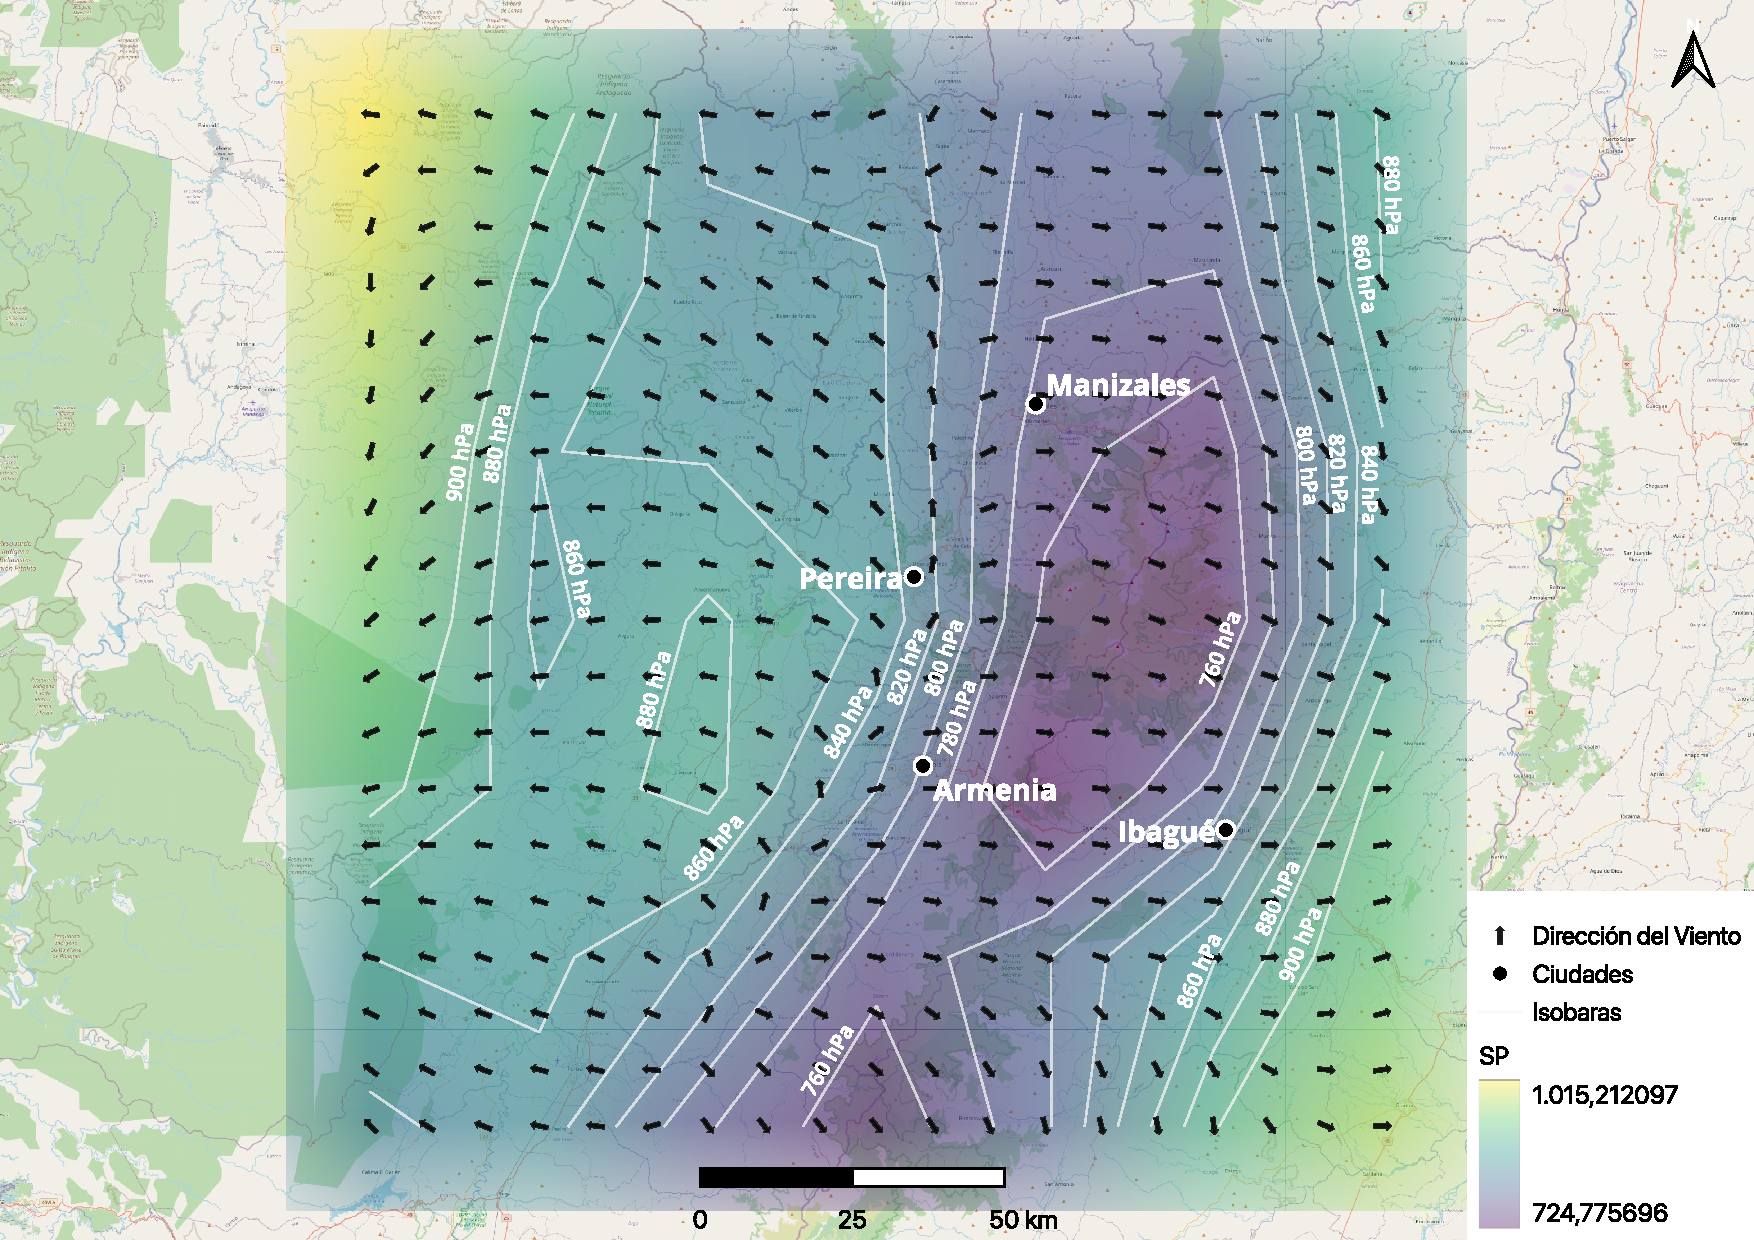
\includegraphics[width=\textwidth]{../../results/plots/mapa_press_qgis.pdf}
		\caption{Presión superficial, isobaras y viento a $10$\,m.}
		\label{fig:mapa_presion_viento}
	\end{subfigure}
	\hfill
	\begin{subfigure}[t]{0.49\textwidth}
		\centering
		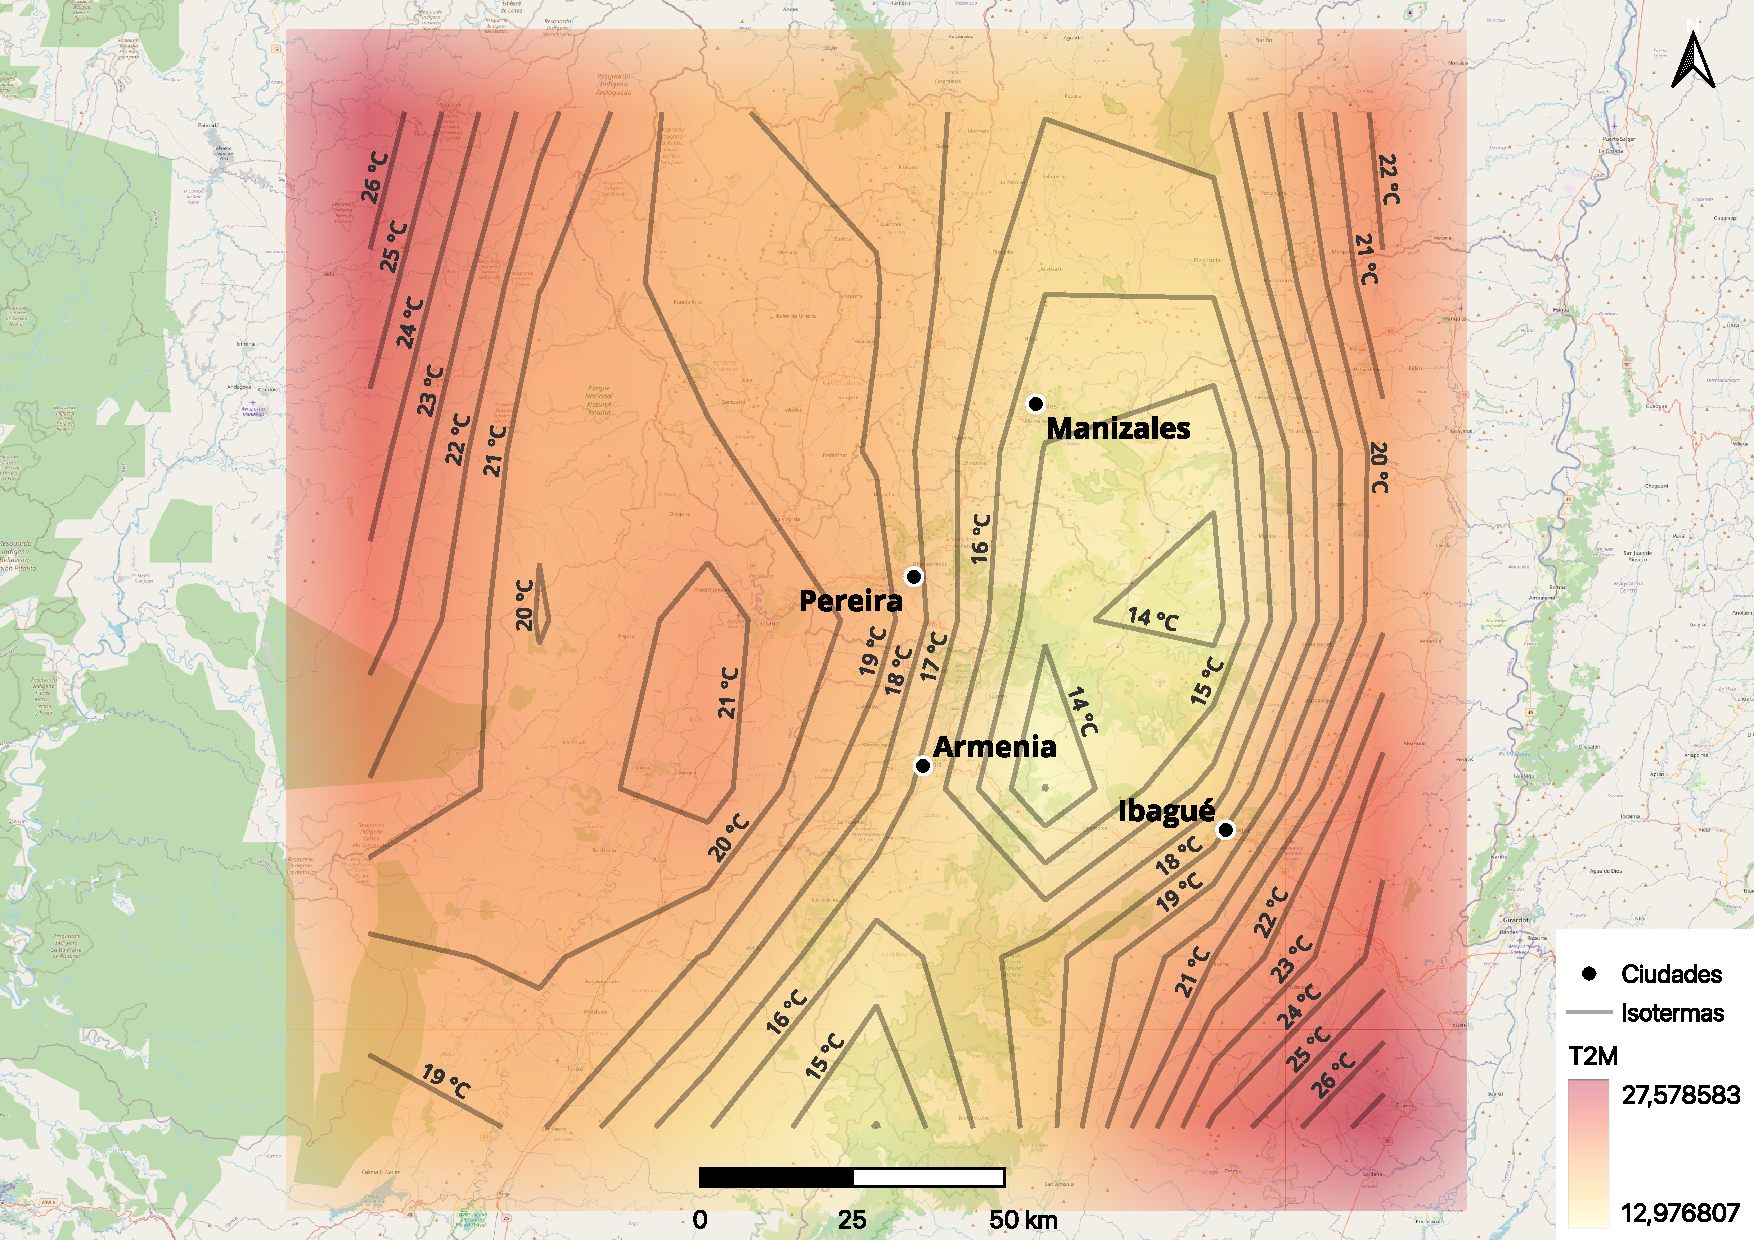
\includegraphics[width=\textwidth]{../../results/plots/mapa_temp_qgis.pdf}
		\caption{Temperatura del aire a $2$\,m.}
		\label{fig:mapa_temperatura}
	\end{subfigure}
	\caption{Campos climatológicos medios 1996--2025. Elaborados
		en QGIS con datos ERA5 ($0.25^{\circ}$, promedios mensuales).}
	\label{fig:mapas_climatologicos}
\end{figure}

El campo de presión superficial (Figura~\ref{fig:mapa_presion_viento})
refleja directamente la variación topográfica de la región. La
presión disminuye desde valores cercanos a $1\,015$\,hPa en las
zonas de menor elevación hasta valores mínimos sobre las cumbres
de la Cordillera Central, patrón coherente con la ley hidrostática.
La presión media regional es de $\sim\!848$\,hPa, consistente con
una elevación efectiva de $\sim\!1\,500$\,m s.n.m.

Los vectores de viento a $10$\,m muestran una circulación débil
en toda la región, con magnitudes inferiores a
$0.8\,\mathrm{m\,s^{-1}}$, característica de la zona de calmas
ecuatoriales. Los flujos tienden a seguir la orientación de los
valles interandinos, evidenciando el control orográfico sobre la
circulación superficial.

El campo de temperatura (Figura~\ref{fig:mapa_temperatura}) exhibe
un gradiente espacial marcado, controlado enteramente por la
topografía. Los valores más altos ($>\!26$\,°C) se localizan en
los fondos de los valles del río Cauca al oeste y del río
Magdalena al este, mientras que los valores más bajos
($<\!14$\,°C) corresponden a las cumbres de la Cordillera
Central. El gradiente horizontal de temperatura entre valles y
cimas supera los $12$\,°C en menos de $50$\,km de distancia
horizontal.

\section{Aproximación Geostrófica}
\label{sec:geostrofia}

\subsection{Formulación}

La aproximación geostrófica establece que, lejos de la superficie
y en ausencia de fricción, el viento horizontal resulta del
equilibrio entre la fuerza de gradiente de presión y la fuerza
de Coriolis:

\begin{equation}
	\mathbf{v}_g = \frac{1}{f}\,\hat{k} \times \nabla_p \Phi,
	\label{eq:geostrofico}
\end{equation}

donde $\Phi = gz$ es el geopotencial, $f = 2\Omega\sin\varphi$
el parámetro de Coriolis y $\hat{k}$ el vector unitario vertical.
En componentes:

\begin{equation}
	u_g = -\frac{1}{f}\frac{\partial \Phi}{\partial y}, \qquad
	v_g =  \frac{1}{f}\frac{\partial \Phi}{\partial x}.
	\label{eq:ug_vg}
\end{equation}

Los gradientes horizontales de $\Phi$ se calcularon mediante
diferencias finitas centradas en coordenadas esféricas, con
un suavizado gaussiano previo ($\sigma = 1$ píxel) para
reducir el ruido numérico inherente a la grilla de solo
$7 \times 7$ puntos.

\subsection{Resultados y métricas de evaluación}

La Figura~\ref{fig:geo_comparacion} muestra la comparación
entre el viento ERA5 y el viento geostrófico calculado en el
nivel de menor RMSE vectorial, y la Figura~\ref{fig:geo_rmse}
presenta las métricas para los 14 niveles de presión disponibles.

\begin{figure}[H]
	\centering
	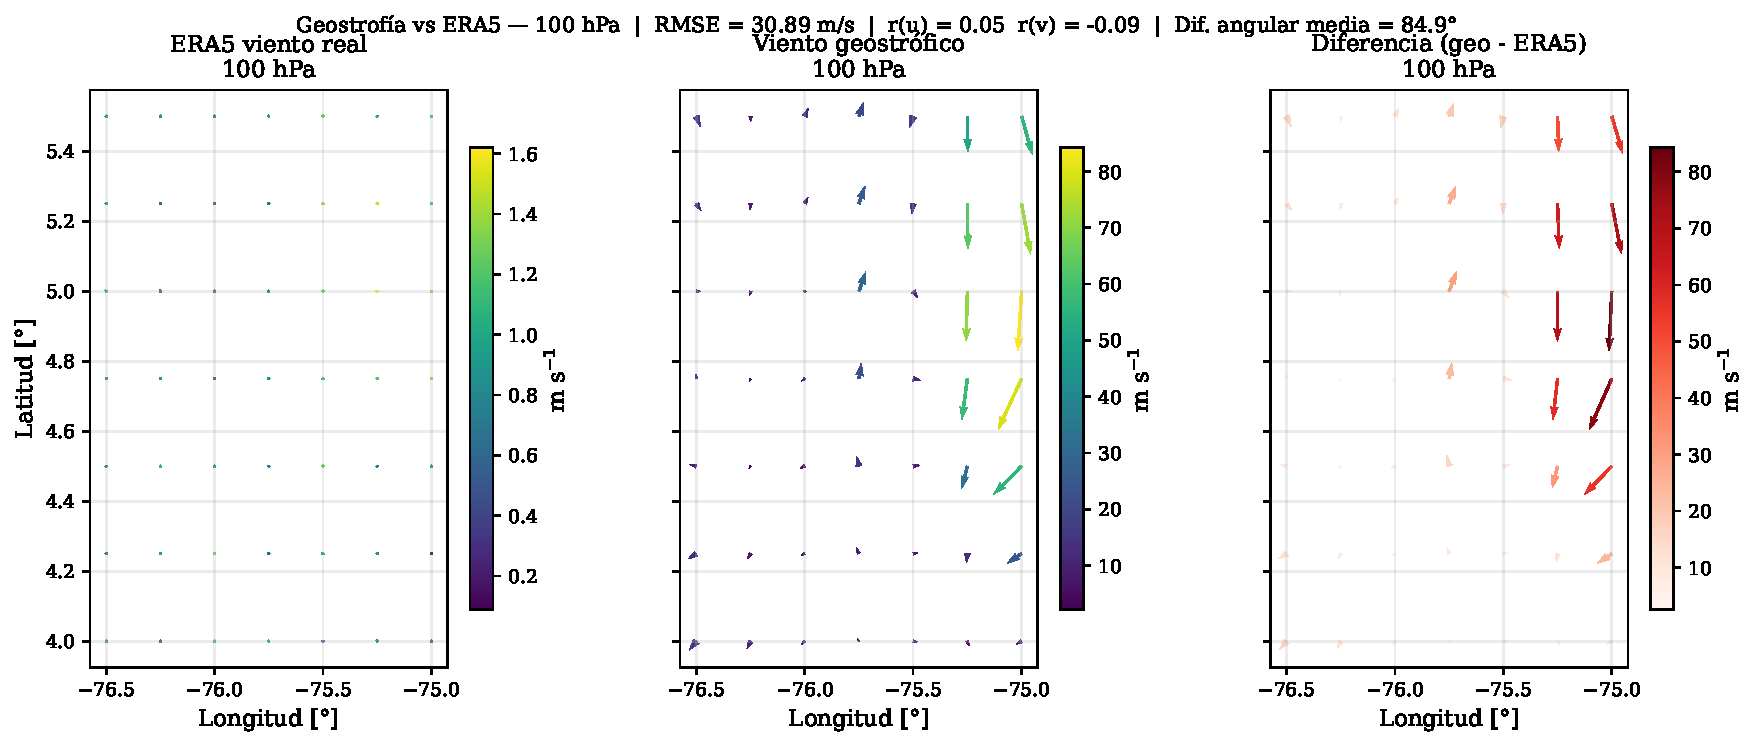
\includegraphics[width=\textwidth]{../../results/plots/04_geostrofia_comparacion.pdf}
	\caption{Comparación del viento ERA5 (izquierda), viento
		geostrófico calculado (centro) y diferencia vectorial
		(derecha) en el nivel de $100$\,hPa. El color indica la
		rapidez en m\,s$^{-1}$.}
	\label{fig:geo_comparacion}
\end{figure}

\begin{figure}[H]
	\centering
	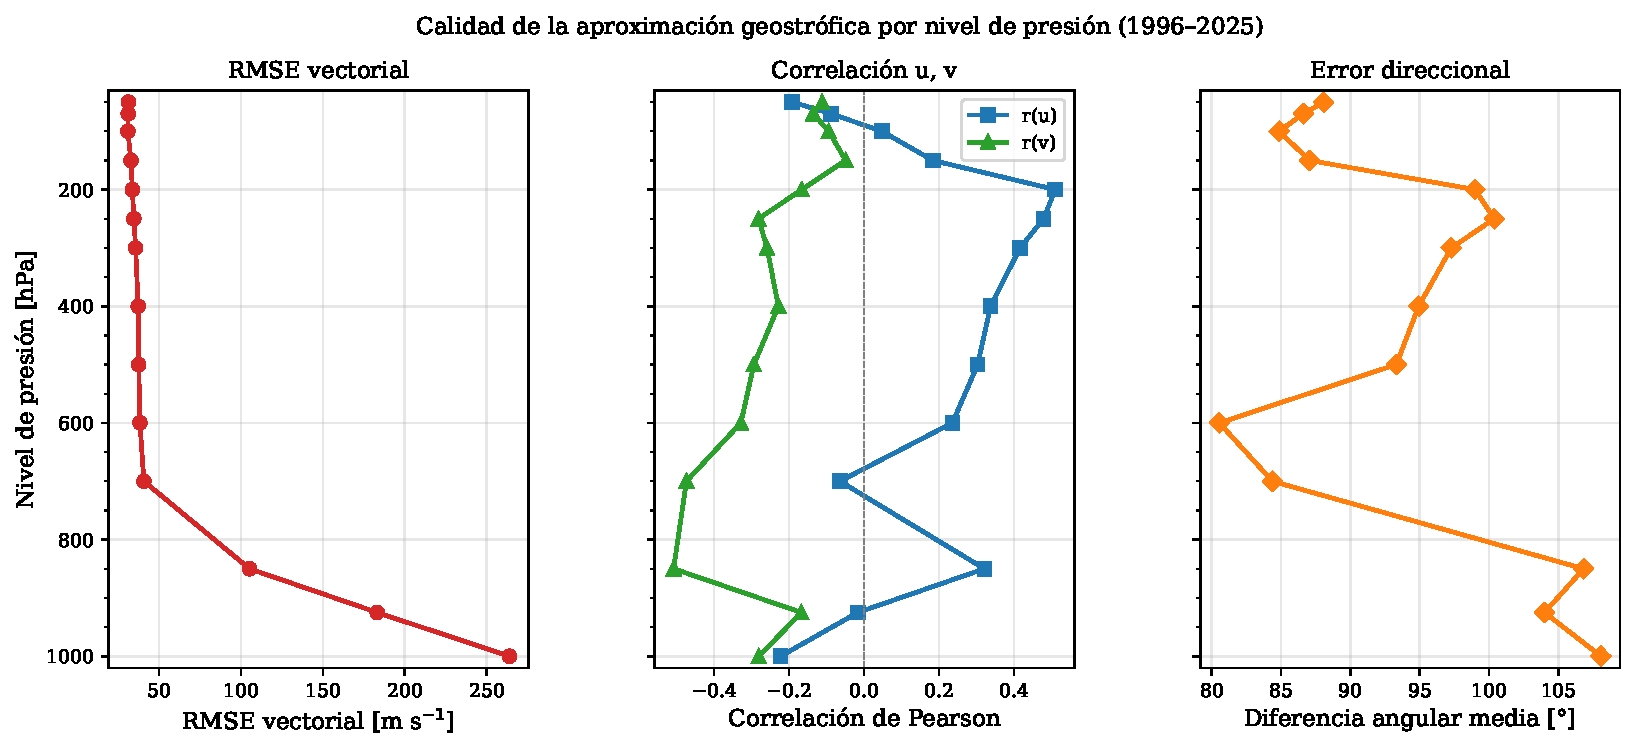
\includegraphics[width=\textwidth]{../../results/plots/04_geostrofia_rmse_por_nivel.pdf}
	\caption{RMSE vectorial, correlación de Pearson ($r$) y
		diferencia angular media entre el viento ERA5 y el
		geostrófico, en función del nivel de presión.}
	\label{fig:geo_rmse}
\end{figure}

La Tabla~\ref{tab:geo_metricas} resume las métricas en todos
los niveles. El RMSE vectorial decrece con la altura desde
$264$\,m\,s$^{-1}$ en $1\,000$\,hPa hasta $\sim\!31$\,m\,s$^{-1}$
en $100$\,hPa, pero en ningún nivel se alcanza una
aproximación razonable: el viento geostrófico calculado
supera al ERA5 entre 24 y 443 veces en rapidez, las
correlaciones son próximas a cero o negativas en ambas
componentes, y la diferencia angular media ronda los
$85$--$108^{\circ}$, indicando que los vectores son
prácticamente perpendiculares o antiparalelos.

\begin{table}[H]
	\centering
	\caption{Métricas de la aproximación geostrófica por
		nivel de presión. $\bar{v}_{\text{ERA5}}$ y
		$\bar{v}_g$ son las rapideces medias del viento real
		y geostrófico respectivamente.}
	\label{tab:geo_metricas}
	\small
	\begin{tabular}{rcccccc}
		\toprule
		$p$ (hPa) & RMSE (m\,s$^{-1}$) & $r(u)$ & $r(v)$
		& $\bar{v}_{\text{ERA5}}$ & $\bar{v}_g$ & $\Delta\theta$ (°) \\
		\midrule
		1000 & 263.98 & $-0.22$ & $-0.28$ & 0.52 & 230.4 & 108.1 \\
		925 & 183.17 & $-0.02$ & $-0.17$ & 0.61 & 159.3 & 104.0 \\
		850 & 105.20 & $+0.32$ & $-0.51$ & 1.00 &  85.9 & 106.8 \\
		700 &  40.68 & $-0.06$ & $-0.47$ & 2.22 &  31.4 &  84.4 \\
		600 &  38.28 & $+0.24$ & $-0.33$ & 3.91 &  27.6 &  80.6 \\
		500 &  37.52 & $+0.30$ & $-0.29$ & 4.62 &  25.7 &  93.3 \\
		400 &  37.20 & $+0.34$ & $-0.23$ & 4.15 &  25.2 &  94.9 \\
		300 &  35.62 & $+0.42$ & $-0.26$ & 3.31 &  23.9 &  97.3 \\
		250 &  34.54 & $+0.48$ & $-0.28$ & 2.81 &  23.2 & 100.4 \\
		200 &  33.62 & $+0.51$ & $-0.17$ & 1.54 &  23.1 &  99.0 \\
		150 &  32.78 & $+0.18$ & $-0.05$ & 0.86 &  22.5 &  87.1 \\
		100 &  30.89 & $+0.05$ & $-0.09$ & 0.90 &  21.5 &  84.9 \\
		70 &  31.12 & $-0.09$ & $-0.14$ & 1.72 &  21.6 &  86.6 \\
		50 &  31.25 & $-0.19$ & $-0.11$ & 1.75 &  21.7 &  88.1 \\
		\bottomrule
	\end{tabular}
\end{table}

Los resultados demuestran que la aproximación geostrófica
no es válida en esta región. Las causas son físicas y
geométricas, y se relacionan directamente con los hallazgos
del ítem anterior:

\begin{enumerate}
	\item \textbf{Latitud tropical.} El parámetro de Coriolis
	en la región es $f \approx 1.0$--$1.4 \times 10^{-5}$\,rad\,s$^{-1}$,
	entre 5 y 10 veces menor que en latitudes medias. Al
	calcular $u_g = -(1/f)\,\partial\Phi/\partial y$, cualquier
	error o variación real en el gradiente de geopotencial
	se amplifica por el mismo factor, produciendo vientos
	geostróficos irrealmente grandes.
	
	\item \textbf{Dominio pequeño y gradientes débiles.}
	La región cubre solo $1.5^{\circ} \times 1.5^{\circ}$
	con $7 \times 7$ puntos. El rango de variación del
	geopotencial en $500$\,hPa es de apenas $\sim\!209$\,m$^2$\,s$^{-2}$
	($\sim\!21$\,m geopotenciales) sobre toda la grilla.
	Las diferencias finitas sobre tan pocos puntos introducen
	errores numéricos comparables o superiores a la señal física.
	
	\item \textbf{Forzamiento ageostrófico.} Como se observó
	en la Sección~\ref{sec:climatologias}, el campo de presión
	superficial está dominado por la topografía andina. La
	circulación real responde a forzamientos orográficos,
	térmicos y friccionales que la aproximación geostrófica
	ignora por construcción.
\end{enumerate}

En latitudes tropicales, el número de Rossby
$Ro = U/(fL) \gg 1$, lo que indica que los términos
inerciales dominan sobre la fuerza de Coriolis y el
equilibrio geostrófico no se establece. La aproximación
solo es fisicamente justificable para $Ro \ll 1$, condición
que se cumple típicamente en latitudes superiores a
$\sim\!30^{\circ}$.

\section{Perfil Vertical de Temperatura}
\label{sec:perfil}

El perfil vertical de temperatura de la región se construyó a
partir de los datos ERA5 en niveles de presión (Sección~\ref{sec:datos}).
Para cada uno de los 14 niveles disponibles se calculó el
promedio climatológico multianual 1996--2025 y el promedio
espacial regional ponderado por $\cos(\varphi)$, obteniendo
así 14 pares $(z, T)$ donde $z$ es la altura geopotencial
media ($z = \Phi/g$) y $T$ la temperatura absoluta media.
Las alturas resultantes cubren desde $116$\,m ($1\,000$\,hPa)
hasta $20\,595$\,m ($50$\,hPa).

El perfil regional se comparó punto a punto con el perfil ISA
calculado en la Sección~\ref{sec:isa}, interpolando la ISA a
las alturas geopotenciales ERA5 mediante interpolación lineal.

La Figura~\ref{fig:perfil_temperatura} muestra los dos perfiles
superpuestos y la Figura~\ref{fig:perfil_diferencia} la
diferencia $\Delta T = T_{\text{ERA5}} - T_{\text{ISA}}$.

\begin{figure}[H]
	\centering
	\begin{subfigure}[t]{0.49\textwidth}
		\centering
		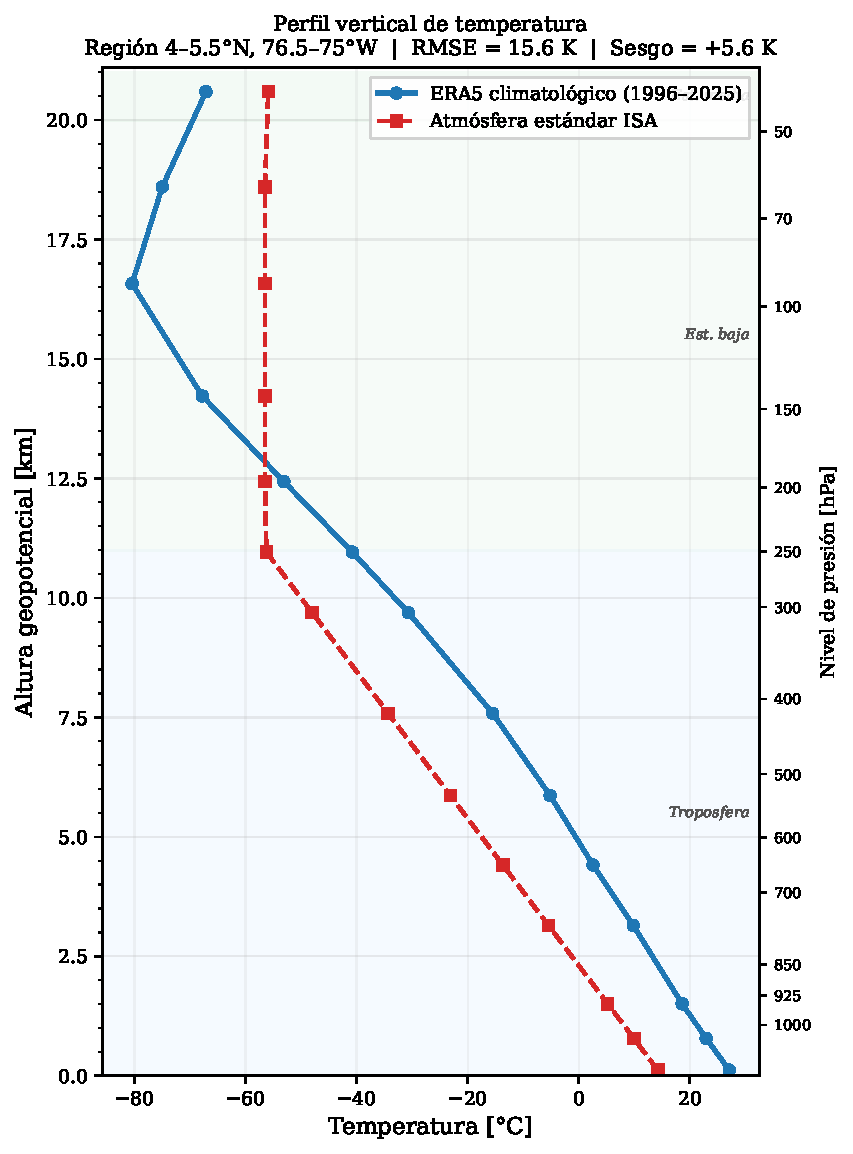
\includegraphics[width=\textwidth]{../../results/plots/05_perfil_vertical_temperatura.pdf}
		\caption{Perfil vertical de temperatura ERA5 vs ISA.}
		\label{fig:perfil_temperatura}
	\end{subfigure}
	\hfill
	\begin{subfigure}[t]{0.42\textwidth}
		\centering
		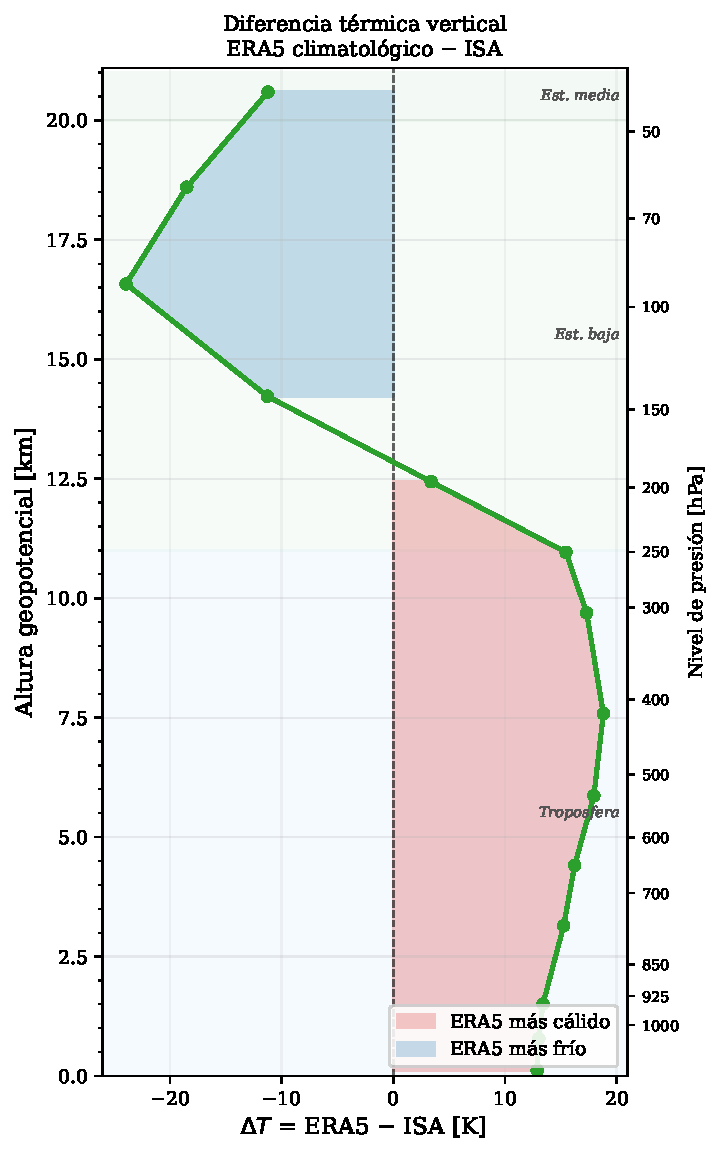
\includegraphics[width=\textwidth]{../../results/plots/05_perfil_vertical_diferencia.pdf}
		\caption{Diferencia térmica respecto al perfil ISA.}
		\label{fig:perfil_diferencia}
	\end{subfigure}
	\caption{Comparación entre el perfil vertical regional derivado de ERA5 y la atmósfera estándar ISA, junto con la diferencia de temperatura entre ambos perfiles.}
	\label{fig:perfiles_combinados}
\end{figure}

Las métricas globales de la comparación son:
$\text{RMSE} = 15.6$\,K, sesgo medio $= +5.6$\,K
(ERA5 sistemáticamente más cálido que la ISA en promedio)
y $\text{MAE} = 14.9$\,K.

El perfil regional difiere de la ISA de forma sistemática y
físicamente interpretable en tres tramos:

\begin{enumerate}
	\item \textbf{Troposfera ($0$--$12$\,km): ERA5 consistentemente
		más cálido.} La diferencia crece desde $+12.9$\,K en
	superficie hasta un máximo de $+18.8$\,K a $7\,585$\,m
	($400$\,hPa). Este calentamiento generalizado es el resultado
	esperado para una región tropical: la ISA está calibrada para
	latitudes medias ($\sim\!45^{\circ}$\,N), donde las
	temperaturas troposféricas son significativamente más bajas
	que en el trópico. La temperatura superficial regional media
	($\sim\!27$\,°C) supera en casi $13$\,K la temperatura de
	referencia de la ISA ($15$\,°C).
	
	\item \textbf{Tropopausa tropical ($\sim\!12$--$16$\,km):
		transición de caliente a frío.} La diferencia disminuye
	rápidamente y cambia de signo cerca de $12.4$\,km
	($200$\,hPa, $\Delta T = +3.4$\,K). Este nivel corresponde
	aproximadamente a la tropopausa tropical, que se sitúa más
	alta ($\sim\!16$\,km) que la tropopausa de latitudes medias
	($\sim\!11$\,km) definida en la ISA.
	
	\item \textbf{Estratosfera baja ($>\!16$\,km): ERA5 más frío.}
	A partir de $100$\,hPa ($16.6$\,km), ERA5 es más frío que la
	ISA en hasta $23.9$\,K. La ISA asume una capa isotérmica a
	$216.65$\,K ($-56.5$\,°C) en la estratosfera baja, mientras
	que el perfil tropical real alcanza temperaturas de hasta
	$-80$\,°C cerca de la tropopausa fría tropical, uno de los
	puntos más fríos de la atmósfera terrestre.
\end{enumerate}

En conjunto, los resultados confirman que la Atmósfera Estándar
ISA es una aproximación útil como referencia global, pero
subestima sistemáticamente la temperatura troposférica en
regiones tropicales y sobreestima la temperatura en la
tropopausa y estratosfera baja. Para aplicaciones que requieran
precisión en esta región, el perfil climatológico ERA5 es
significativamente más representativo.

\section{Conclusiones}
\label{sec:conclusiones}

Este trabajo evaluó tres aproximaciones fundamentales de la
dinámica y termodinámica atmosférica en el contexto del Eje
Cafetero colombiano, usando el reanálisis ERA5 como referencia
observacional para el período 1996--2025. Los principales
hallazgos son los siguientes. La Atmósfera Estándar ISA fue implementada exitosamente
para las siete capas oficiales hasta $86$\,km, con errores
inferiores al $0.04$\,\% respecto a la tabla ISO~2533:1975 en
el rango $0$--$71$\,km. Los perfiles de presión y densidad
muestran el decaimiento cuasiexponencial esperado, mientras
que el perfil de temperatura exhibe la estructura en capas
característica con cambios de gradiente en cada interfaz.
La ISA constituye una referencia numérica sólida para el
rango troposférico de interés en este trabajo.

La aproximación geostrófica falla sistemáticamente en
la región de estudio en todos los niveles de presión evaluados.
El RMSE vectorial mínimo alcanzado fue de $30.9$\,m\,s$^{-1}$
(nivel de $100$\,hPa), frente a una rapidez media ERA5 de
apenas $0.9$\,m\,s$^{-1}$ en ese nivel, lo que representa un
error relativo superior al $2\,200$\,\%. Las correlaciones entre
el viento geostrófico y el ERA5 son próximas a cero o negativas
en todas las capas, y las diferencias angulares medias superan
los $80^{\circ}$ en todos los niveles. Esta falla es atribuible
a tres causas concurrentes: la latitud tropical de la región
($f \approx 1.2 \times 10^{-5}$\,rad\,s$^{-1}$, cinco veces
menor que en latitudes medias), el dominio espacial reducido
($1.5^{\circ} \times 1.5^{\circ}$, $7 \times 7$ puntos) que
amplifica los errores numéricos en el cálculo de gradientes,
y el forzamiento ageostrófico dominante asociado a la
topografía andina. La aproximación geostrófica solo es
físicamente justificable cuando el número de Rossby
$Ro = U/(fL) \ll 1$, condición que no se cumple en regiones
tropicales. El perfil vertical de temperatura regional difiere
de la ISA de forma sistemática y físicamente interpretable.
En la troposfera, ERA5 es consistentemente más cálido que la
ISA en $+13$ a $+19$\,K, reflejo del origen tropical de la
región frente a la calibración de la ISA para latitudes medias.
La tropopausa tropical se sitúa más alta ($\sim\!16$\,km) y
más fría ($-80$\,°C) que la de la ISA ($11$\,km, $-56.5$\,°C),
produciendo una inversión del sesgo en la estratosfera baja
de hasta $-24$\,K. El RMSE global entre ERA5 e ISA es de
$15.6$\,K. Estos resultados confirman que la ISA no es
representativa del clima tropical y que su uso como referencia
en esta región introduce errores sistemáticos significativos.

En síntesis, las tres aproximaciones evaluadas tienen validez
limitada o nula en el contexto tropical andino del Eje
Cafetero. La ISA es útil como referencia teórica pero no
como modelo climático regional. La geostrofía no aplica en
latitudes ecuatoriales con topografía compleja. El perfil
vertical ERA5 es el más representativo de las condiciones
reales de la región y constituye la referencia más adecuada
para estudios de dinámica atmosférica local.

% Bibliografía
\newpage
\bibliographystyle{plainnat}
\bibliography{referencias}

\end{document}
